\subsection{Duration of the Battles}

 \begin{figure}[h]
	\centering	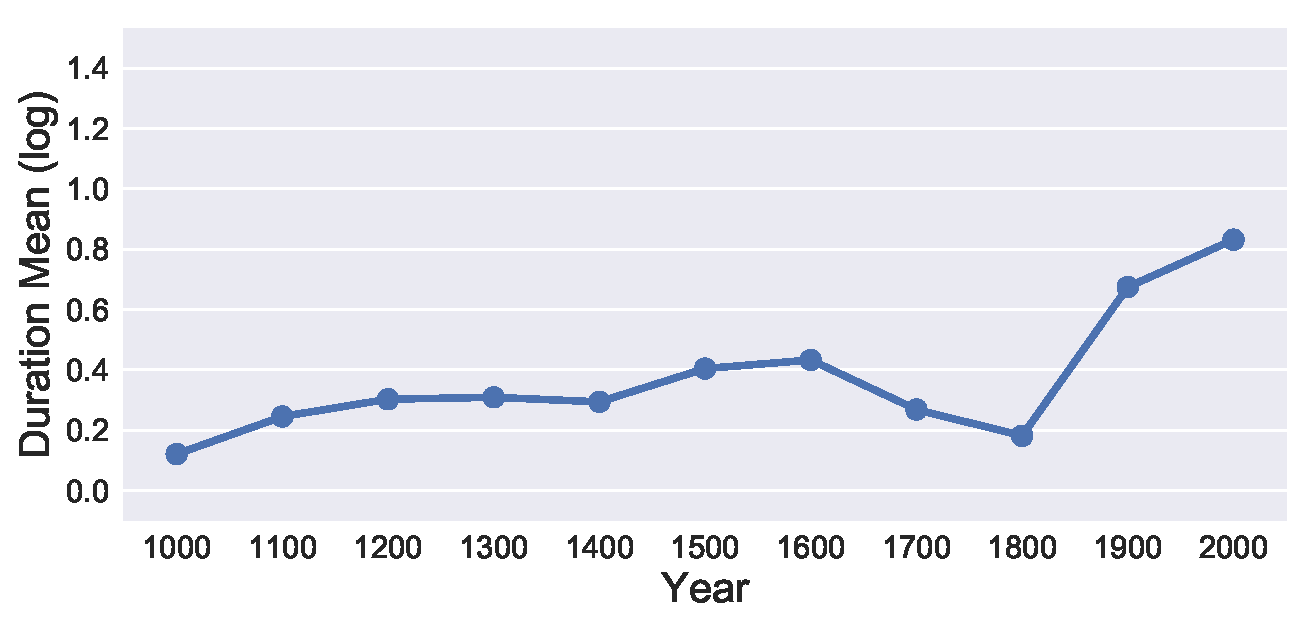
\includegraphics[width=\linewidth]{figures/durThByCent}
	\caption{Mean of the duration of battles in the last thousand years by century on a logarithmic scale.}\label{fig:durThByCent}
	\centering
\end{figure}

\subsection{Evolution of the Casualties}

 \begin{figure}[h]
	\centering	\includegraphics[width=\linewidth]{figures/casuPerCent}
	\caption{Mean of the percentage of casualties in the soldiers.}\label{fig:casuPerCent}
	\centering
\end{figure}

\subsection{Indecisiveness of the Battles}
TODO mettre la bonne figure
 \begin{figure}[h]
	\centering	\includegraphics[width=\linewidth]{figures/casuPerCent}
	\caption{Mean of the percentage of casualties in the soldiers.}\label{fig:casuPerCent}
	\centering
\end{figure}


\subsection{Outcome of the Battle}
David has an idea to test here

\subsection{Years of Battles per Countries}
In Figure \ref{fig:FightingDurationRanking}, we observe that among all the countries, France is the one that fought the most. Nevertheless, the United States, which are a major actor in the international history of battles, were only created in 1776 when they proclaimed their independence. Thus, it is interesting to do the same ranking starting from this year. 
 \begin{figure}[h]
	\subfigure[Duration of battles engagement per country since year 1000.]{\includegraphics*[width=\linewidth]{figures/YearsFightingRanking}} 
	\vspace{-0.5 em}
	\subfigure[Duration of battles engagement per country since year 1775 (USA Independence).]{\includegraphics*[width=\linewidth]{figures/YearsFightingRankingModern}}
	\vspace{-0.1 em}
	\caption{Cumulated duration of battles engagement per country.} 
	\label{fig:FightingDurationRanking}
\end{figure}
 These results tend to support the common belief that the United States are always in war. In fact, as we observe in Figure \ref{fig:USAFightingTimeline}, they were engaged in a at least one battle per year for more than 150 years in 242 years of existence.
 \begin{figure}[h]
 	\centering	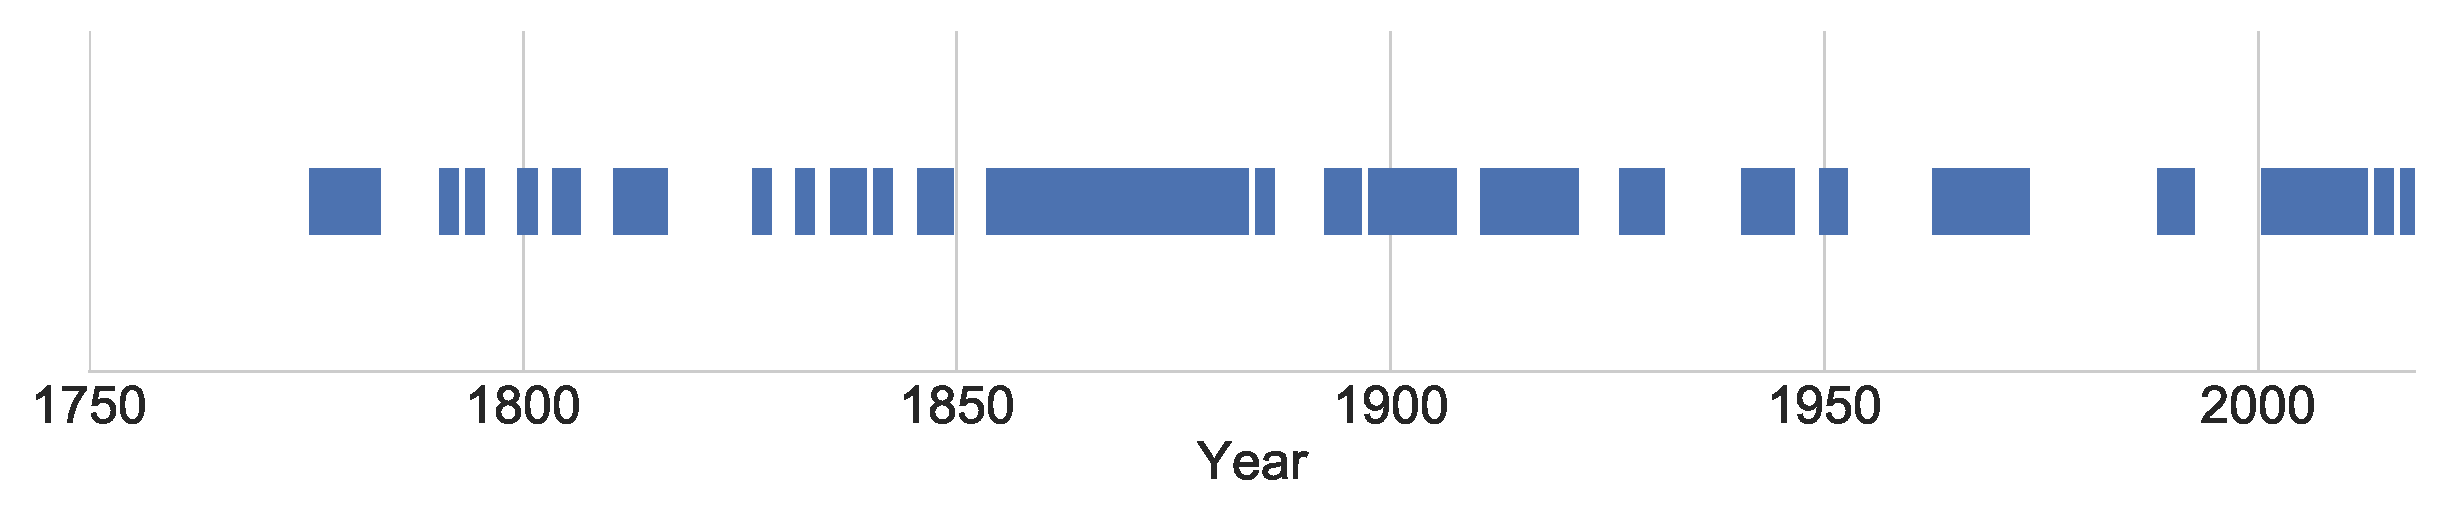
\includegraphics[width=\linewidth]{figures/USAFighting}
 	\caption{Timeline of the USA engagement in battles.}\label{fig:USAFightingTimeline}
 	\centering
 \end{figure}

